\subsubsection{Trachemys --- Sliders}
\begin{center}
\begin{longtabu} to \textwidth {| | p{3.5cm} | X | |}

	\hline
	Taxonomy/Ancestry &
	subfamily Deirochelyinae. 16 species w/ 19 subspecies b/w them. named for how they ``slide" into the water if they sense danger while basking. also known as red-eared terrapins*.
	
	\begin{center} \includegraphics[scale=0.5]{testudines/emydidae/trachemys/tax} \end{center}
	 \\
	\hline
	Size & 
	carapace typically 15-20 cm (6-8 in).
	\\
	\hline
	Color &
	distinct broad stripe extending from right behind eye, slightly curving. the carapace is leaf green in the young, turning dark w/ age. light yellow plastron w/ dark irregular markings in the center of the scutes.
	 \\
	\hline
	Anatomy &
	\begin{itemize}[noitemsep]
		\item the carapace is oval and flattened, w/ a weak keel that is more pronounced in the young
		\item upper carapace contains vertebral scutes forming central elevated portion
		\item relies on middle ear covered by cartilaginous disc; no visible outer ear or external auditory canal
		\item live 20-30 years; shorter in captivity
	\end{itemize}
	 \\
	\hline
	Dimorphism & 
	females larger.
	
	males have longer claws on front feet to hold female during mating. thicker and longer tail holding dark colored, retractable penis.
	
	in the male, the cloaca is beyond the edge of the carapace, while in the female, it is at or under the rear edge of the carapace.
	
	the male's plastron is slightly concave, while the female's is completely flat.
	\\
	\hline
	Behavior & 
	\begin{itemize}[noitemsep]
		\item often seen basking in groups
		\item almost entirely aquatic but bask to maintain body temp.
		\item do not hibernate, but brumate*
			\begin{itemize}[noitemsep]
				\item occasionally rise to surface for food, drink, or air
				\item inactive in October when temp $< 10\circ$C (50$\circ$F) --- enter state of topor and do not eat or defecate, remain motionless, less breathing, may become active during warmer times in winter but return when temp drops
				\item survive anaerobically producing ATP from glycolysis w/ dropped metabolic rate
				\item do not brumate* if captive
			\end{itemize}
	\end{itemize}	
	\\
	\hline
	Habitat & 
	exclusively freshwater, they live in habitats w/ rocks or logs to bask on.
	\\
	\hline
	Distribution & 
	native to the Americas, they range from the US to northern Argentina.
	\\
	\hline
	Feeding Ecology & 
	Young pond sliders tend to be more carnivorous than adults, eating about 70\% animal matter and 30\% plant matter. Adults eat 90\% plant matter and 10\% animal matter. Foods include aquatic insects, snails, tadpoles, crawfish and other crustaceans, and fish. They also eat plants like arrowhead, water lilies, hyacinths, and duck weed. Feeding occurs under water, usually in the early morning or late afternoon.
	
	Pond slider eggs and hatchlings are preyed on by raccoons, skunks, opossums, foxes, and other predators. They are relatively safe from most predators once they reach adult size and while they are in the water. Large predatory fish seem to find the hatchlings difficult to handle and do not tend to eat them. Red-eared sliders may attempt to bite and scratch when harassed, but most pull their head and legs into their shells for protection.
	\\
	\hline
	Reproductive Biology & 
	\begin{itemize}[noitemsep]
		\item mating takes place from March-July
		\item courtship --- male swims around female and flutters claws around her head; if receptive, female swims toward male and sinks to bottom for mating
		\item courtship = 45 min, mating = 10 min
		\item on occasion male appears to be courting another male; may be sign of dominance or preclude fight
		\item post-mating, female spends extra time basking to keep eggs warm. she may change her diet.
		\item can lay 2-30 eggs, up to 5 clutches a year
		\item actual egg fertilization takes place during egg-laying --- female can lay fertile eggs in following season w/o mating
		\item during last weeks of gestation female spends time scratching at ground to find suitable place
		\item Incubation = 59-112 days
		\item hatchling breaks egg w/ egg tooth
		\item may overwinter in nest
		\item new hatchling has yolk sac attached to stomach which will be absorbed; damaging yolk sac = death $\rightarrow$ when relocating eggs, always mark top so they don't get flipped over and let sac strangle baby
	\end{itemize}
	\\
	\hline
	Ecological Role &
	Pond sliders help to control populations of the animals that they consume and affect aquatic vegetation as they graze. Young pond sliders are an important food source for large, aquatic predators.
	\\
	\hline
	Conservation Status & 
	\begin{itemize}[noitemsep]
		\item most commonly traded reptile
		\item when mature, they can bite, which results in them being dumped into the wild
		\item asymptomatic carriers of salmonella; FDA banned selling turtle eggs and turtles w/ carapace length under 4 in (10 cm)
		\item considered significant threat to native turtle species in Australia; high social/economic costs predicted
	\end{itemize}
	\\
	\hline
\end{longtabu}
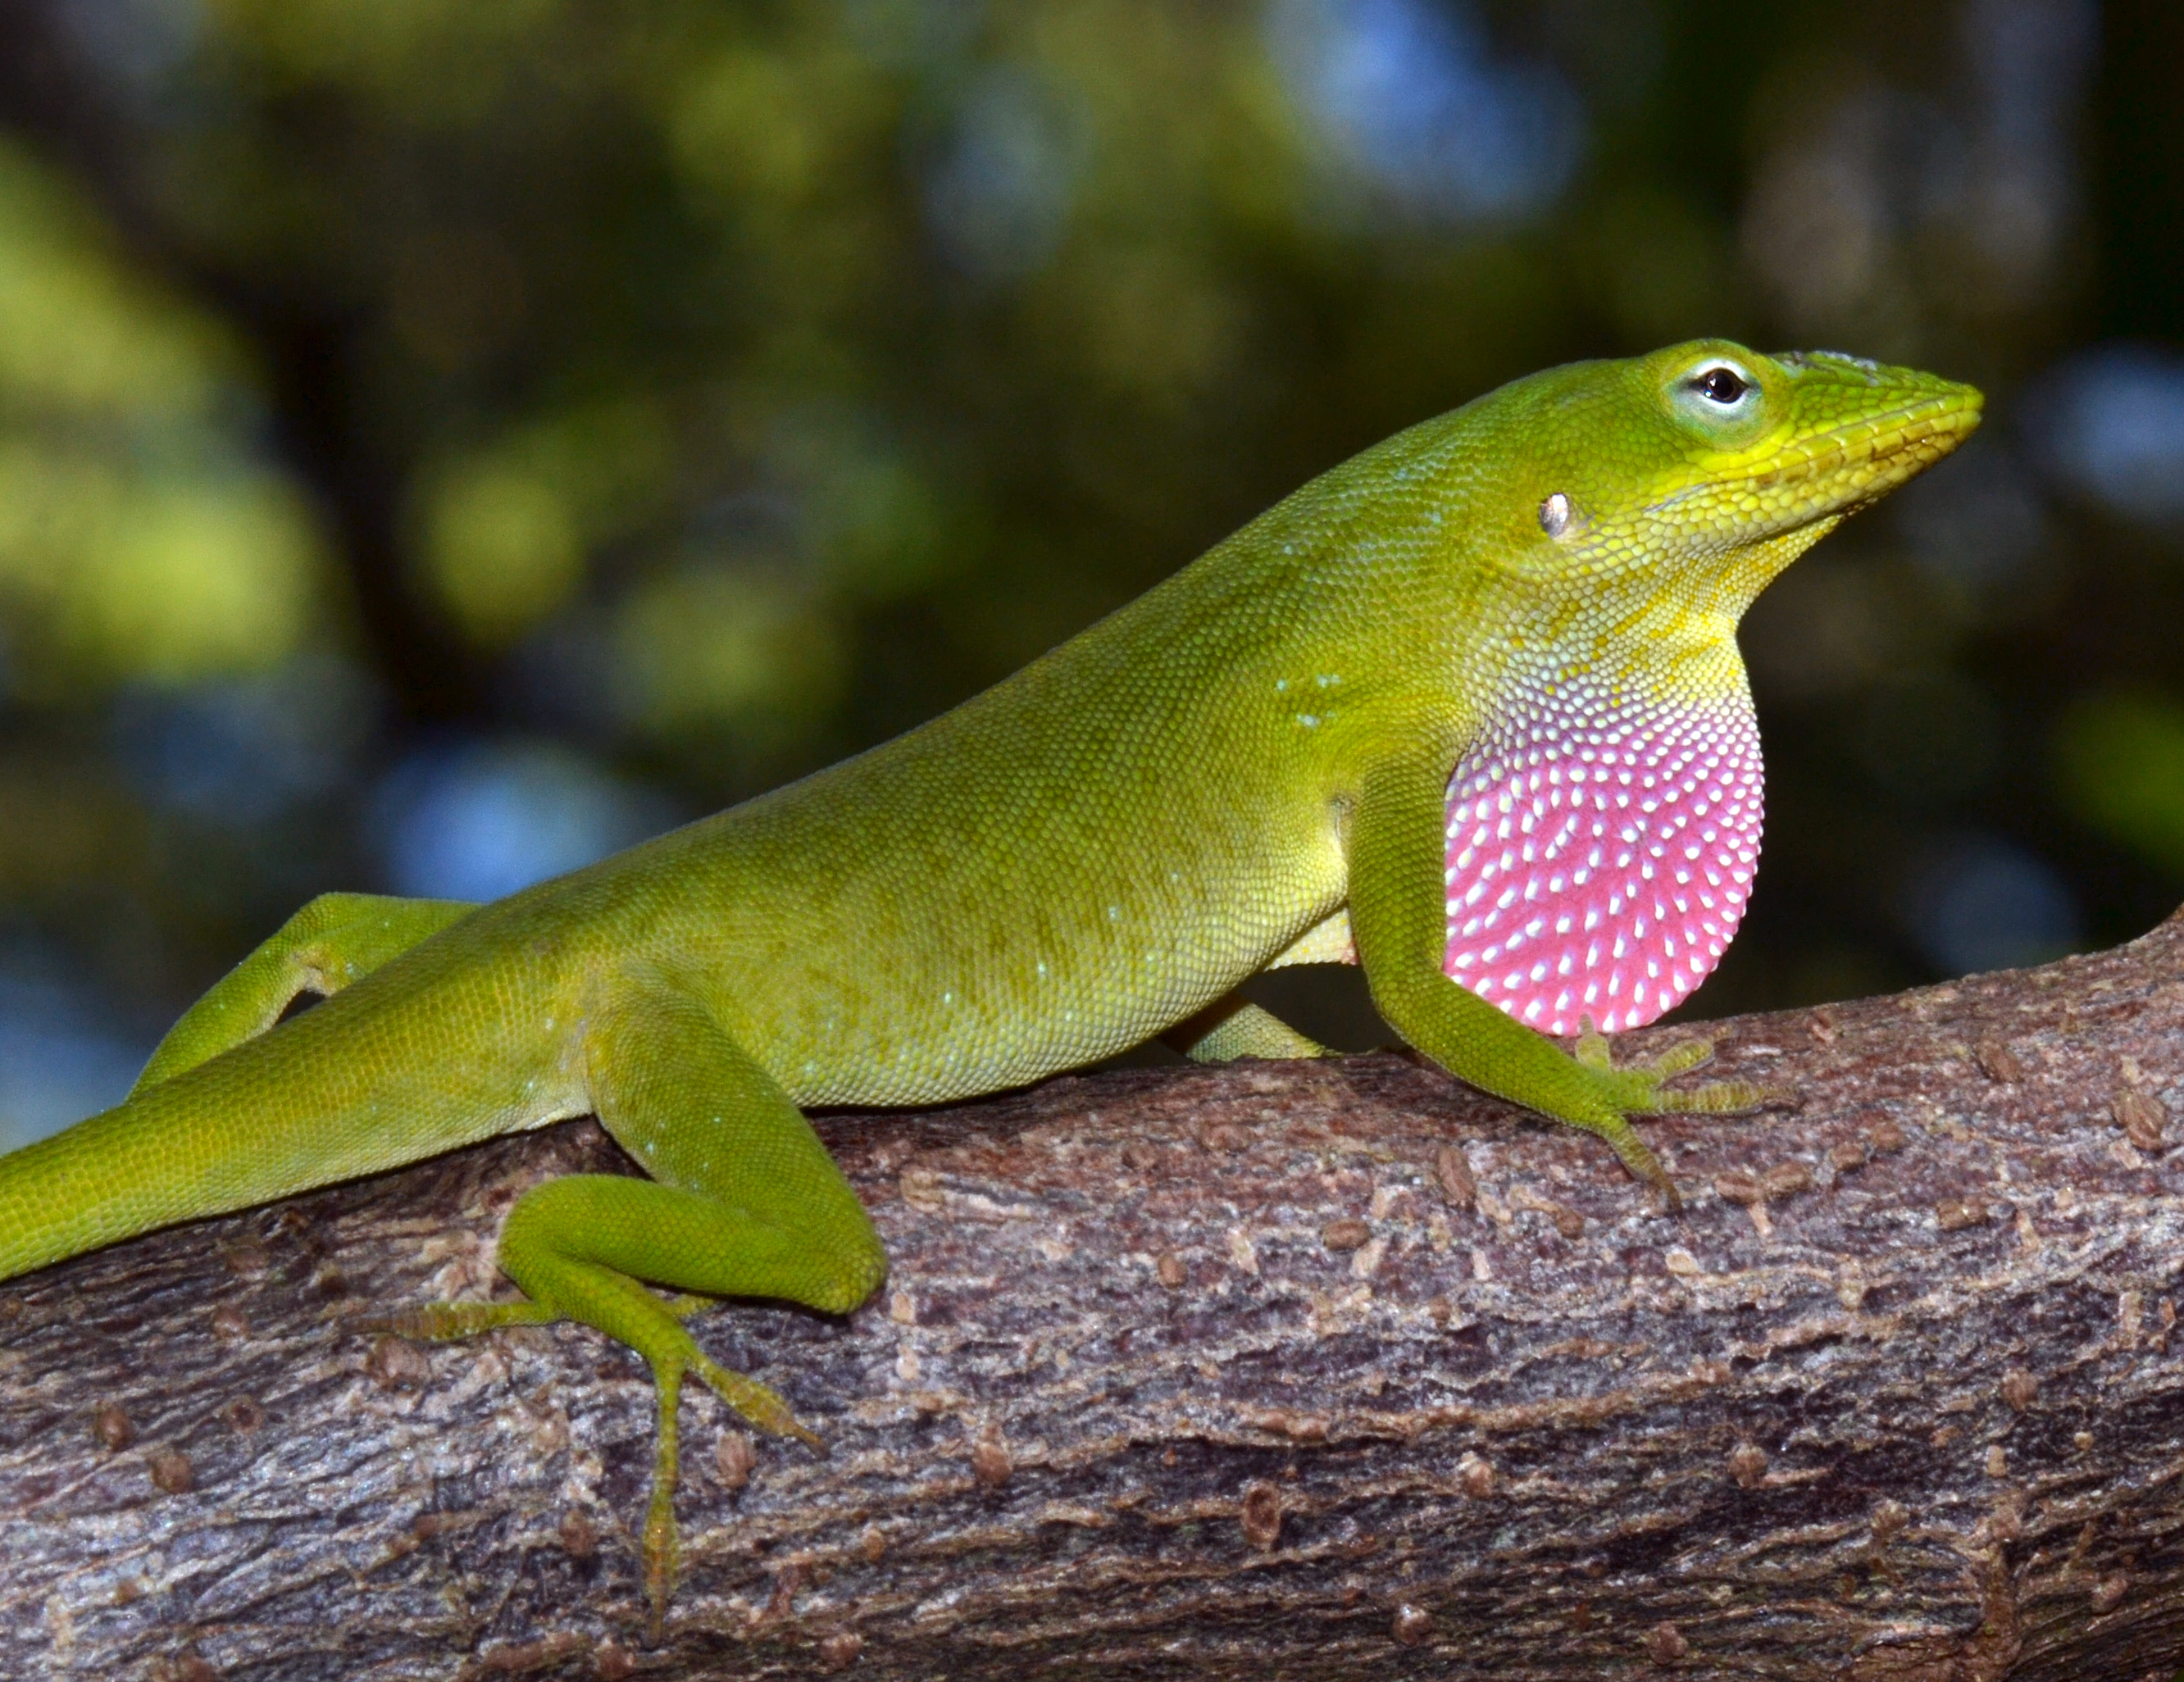
\includegraphics[scale=0.25]{testudines/emydidae/trachemys/1}
\includegraphics[scale=0.75]{testudines/emydidae/trachemys/2}
\end{center}